\documentclass[tikz]{standalone}
\usetikzlibrary{calc}
\usepackage{amssymb}

\tikzset{
  geometry/line/.style={draw=black, line width=0.8pt, line cap=round},
  geometry/aux/.style={draw=black!50, line width=0.5pt, dashed},
  geometry/point/.style={circle, fill=black, inner sep=0pt, minimum size=3.5pt}
}

\begin{document}
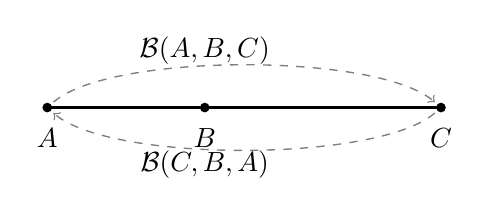
\begin{tikzpicture}
  % Step A & B: Coordinate Initialization
  \coordinate (A) at (0,0);
  \coordinate (C) at (5,0);
  \coordinate (B) at ($(A)!0.4!(C)$);

  % Step C: Primary Line Stroke
  \draw[geometry/line] (A) -- (C);

  % Step D: Elegant Tracking Curves with Absolute Offsets & Padding
  % Top tracking loop (A -> B -> C) sweeping smoothly across the dynamic field
  \draw[geometry/aux, ->, shorten >=3pt, shorten <=3pt]
    (A) .. controls ($(A)+(0.8, 0.7)$) and ($(C)+(-0.8, 0.7)$) .. (C);

  % Bottom tracking loop (C -> B -> A) matching perfectly in symmetry
  \draw[geometry/aux, ->, shorten >=3pt, shorten <=3pt]
    (C) .. controls ($(C)+(-0.8, -0.7)$) and ($(A)+(0.8, -0.7)$) .. (A);

  % Step E: Micro-Tuned Text Labeling (No combined directions)
  \node[above=12pt] at (B) {$\mathcal{B}(A,B,C)$};
  \node[below=12pt] at (B) {$\mathcal{B}(C,B,A)$};

  \node[below=4pt] at (A) {$A$};
  \node[below=4pt] at (B) {$B$};
  \node[below=4pt] at (C) {$C$};

  % Step F: Foreground Point Markers (Drawn last to sit on top of lines)
  \node[geometry/point] at (A) {};
  \node[geometry/point] at (B) {};
  \node[geometry/point] at (C) {};
\end{tikzpicture}

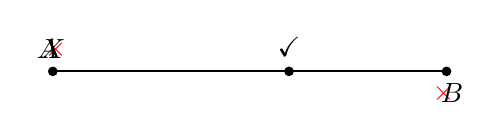
\begin{tikzpicture}
  % Step A: Define base points
  \coordinate (A) at (0,0);
  \coordinate (X) at (3,0);
  \coordinate (B) at (5,0);

  % Step C: Draw the main segment line
  \draw[geometry/line] (A) -- (X) -- (B);

  % Step D: Overlay directional tracking lines and symbols
  \node[above=2pt] at (X) {$\checkmark$};
  \node[right=1pt, above=1pt] at (A) {\textcolor{red}{$\times$}};
  \node[left=1pt, below=1pt] at (B) {\textcolor{red}{$\times$}};

  % Step E: Overlay point markers and labels
  \node[geometry/point] at (A) {};
  \node[geometry/point] at (X) {};
  \node[geometry/point] at (B) {};

  \node[left=2pt, above=1pt] at (A) {$A$};
  \node[right=2pt, below=1pt] at (B) {$B$};
  \node[midway, above=1pt] at (X) {$X$};
\end{tikzpicture}

\end{document}
